%! TEX program = xelatex
%! TEX root = ../root.tex

\section{实验步骤与调试}
\subsection{仿真} 根据已经写好的代码,进行仿真模拟\\
当load指令后紧接着alu指令时,既要stall又要forwarding。
\begin{figure}
	\centering %图片居中
	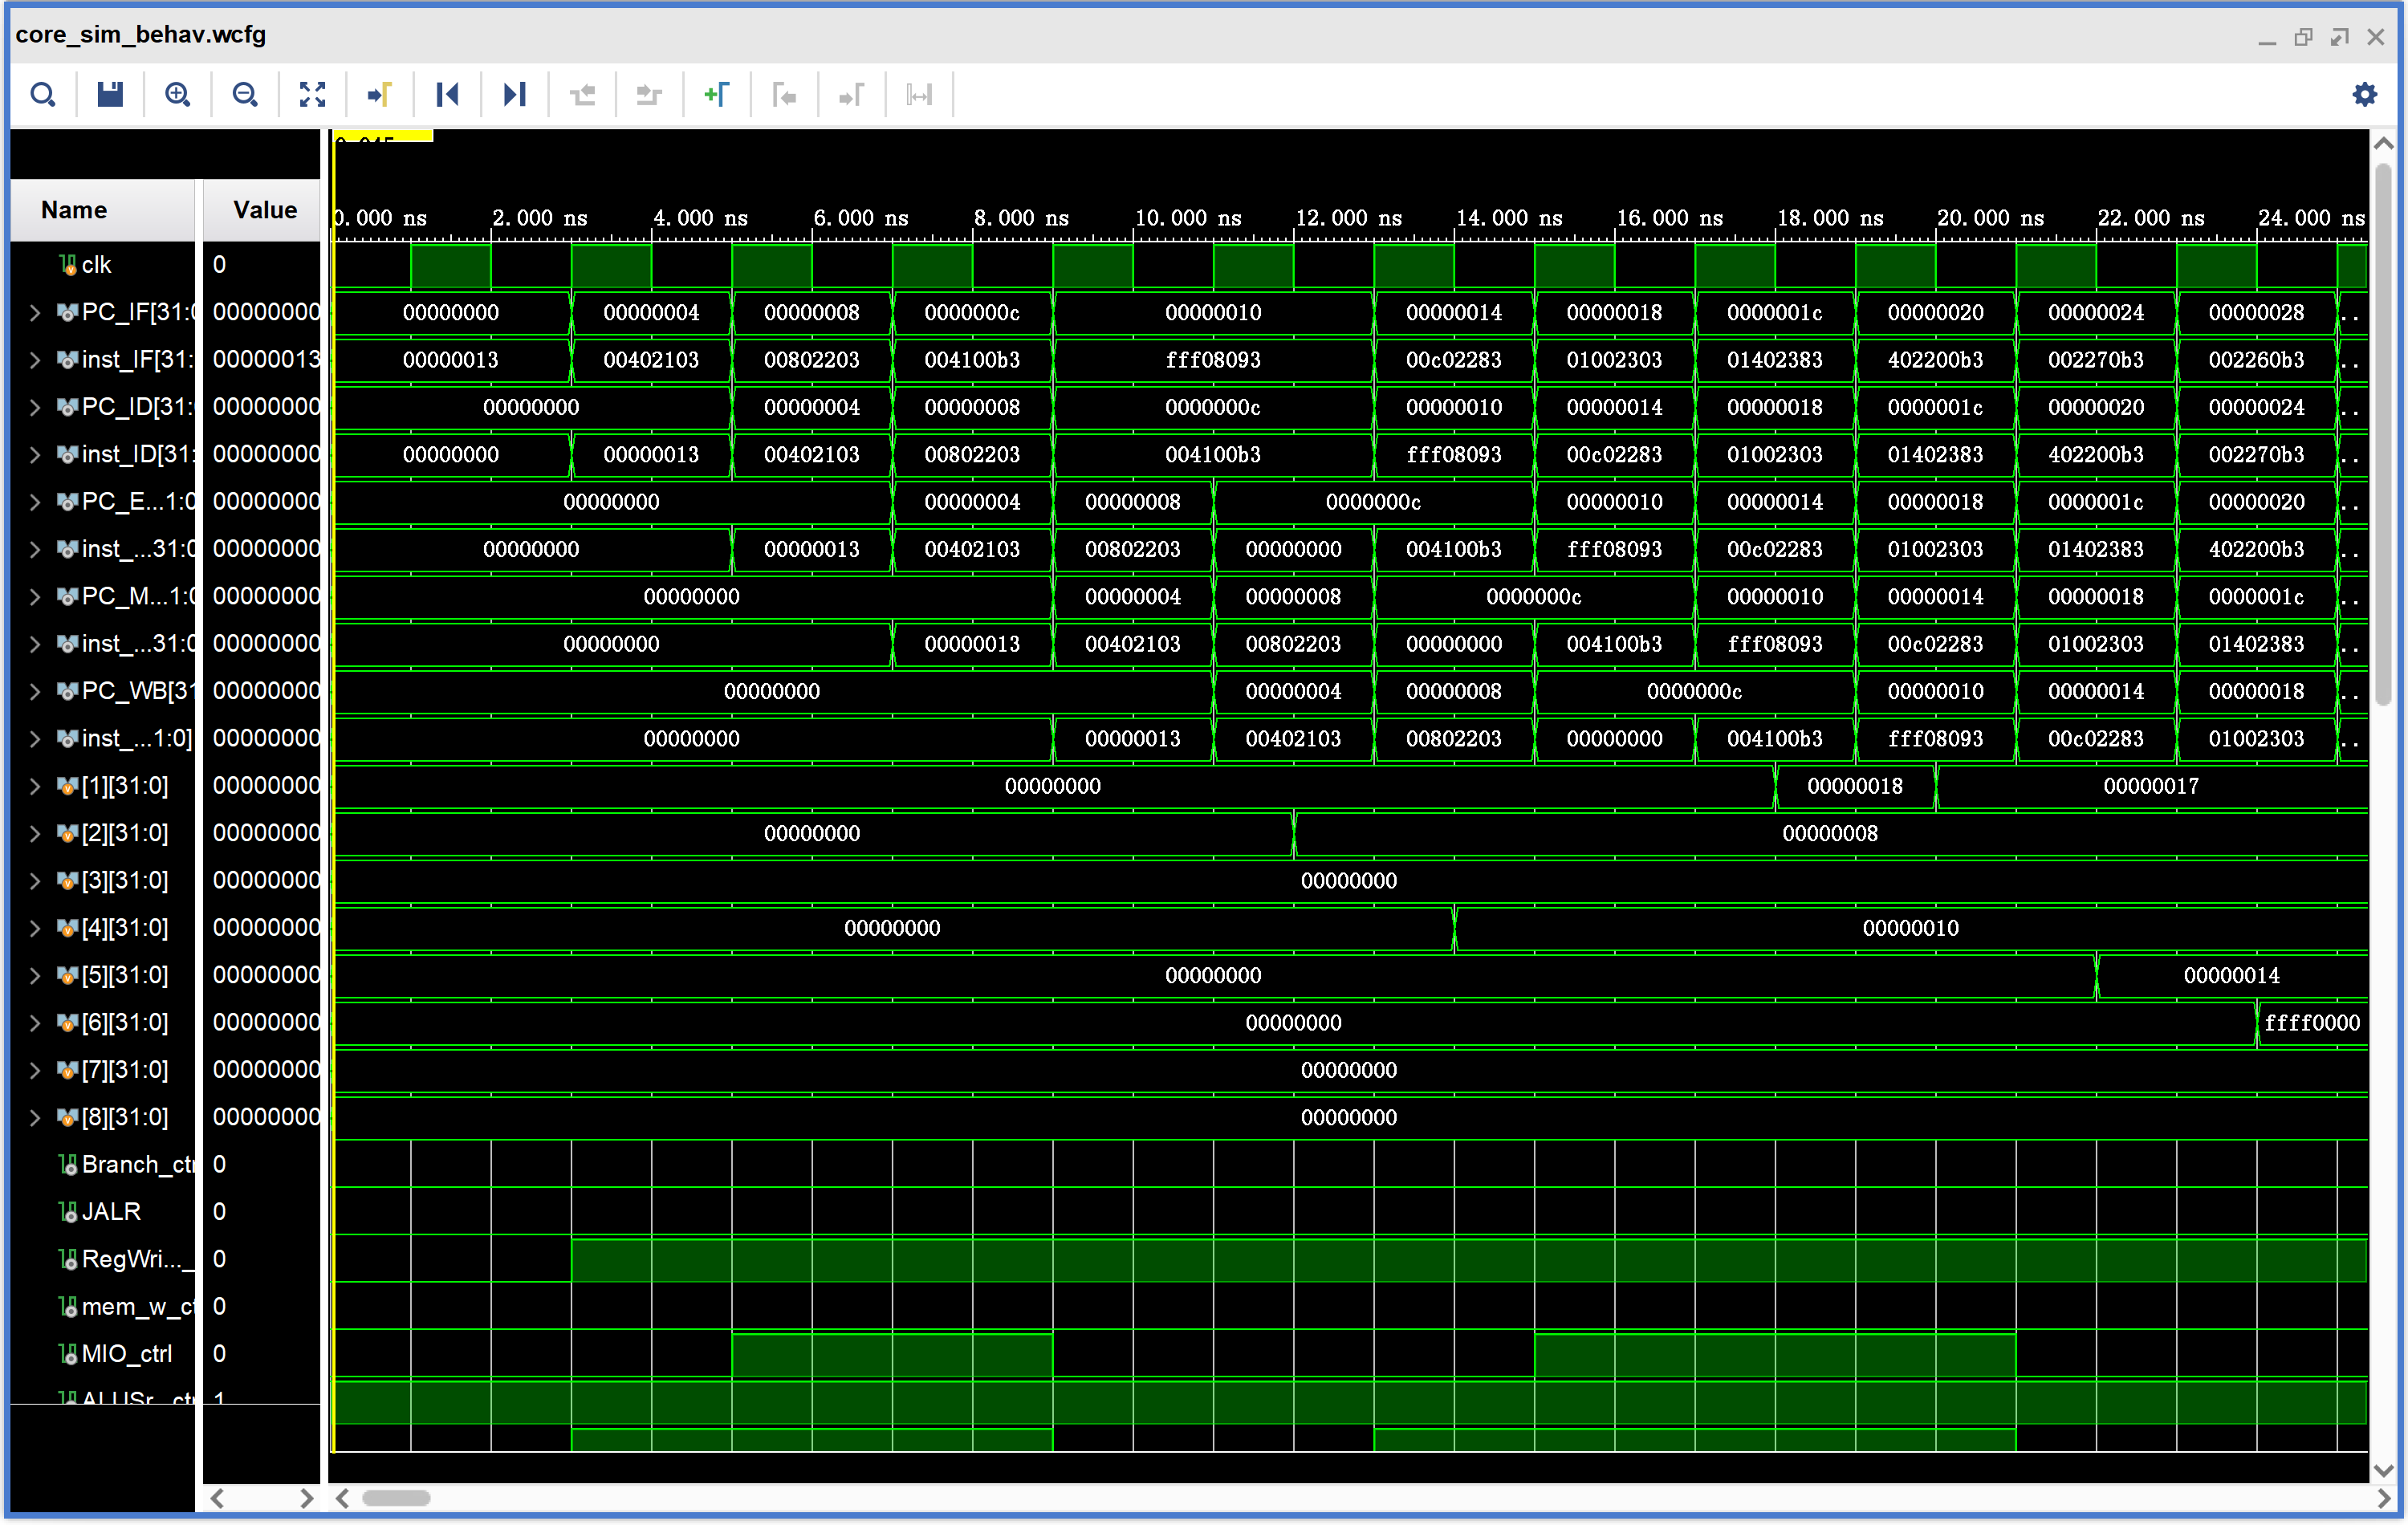
\includegraphics[width=1.0\textwidth]{f1.png} %插入图片,[]中设置图片大小,{}中是图片文件名
	\caption{仿真结果图} %最终文档中希望显示的图片标题
	\label{Fig.3} %用于文内引用的标签
\end{figure}
由图3.3可以验证forwarding功能已经实现。\\
branch指令验证如图3.4
\begin{figure}
	\centering %图片居中
	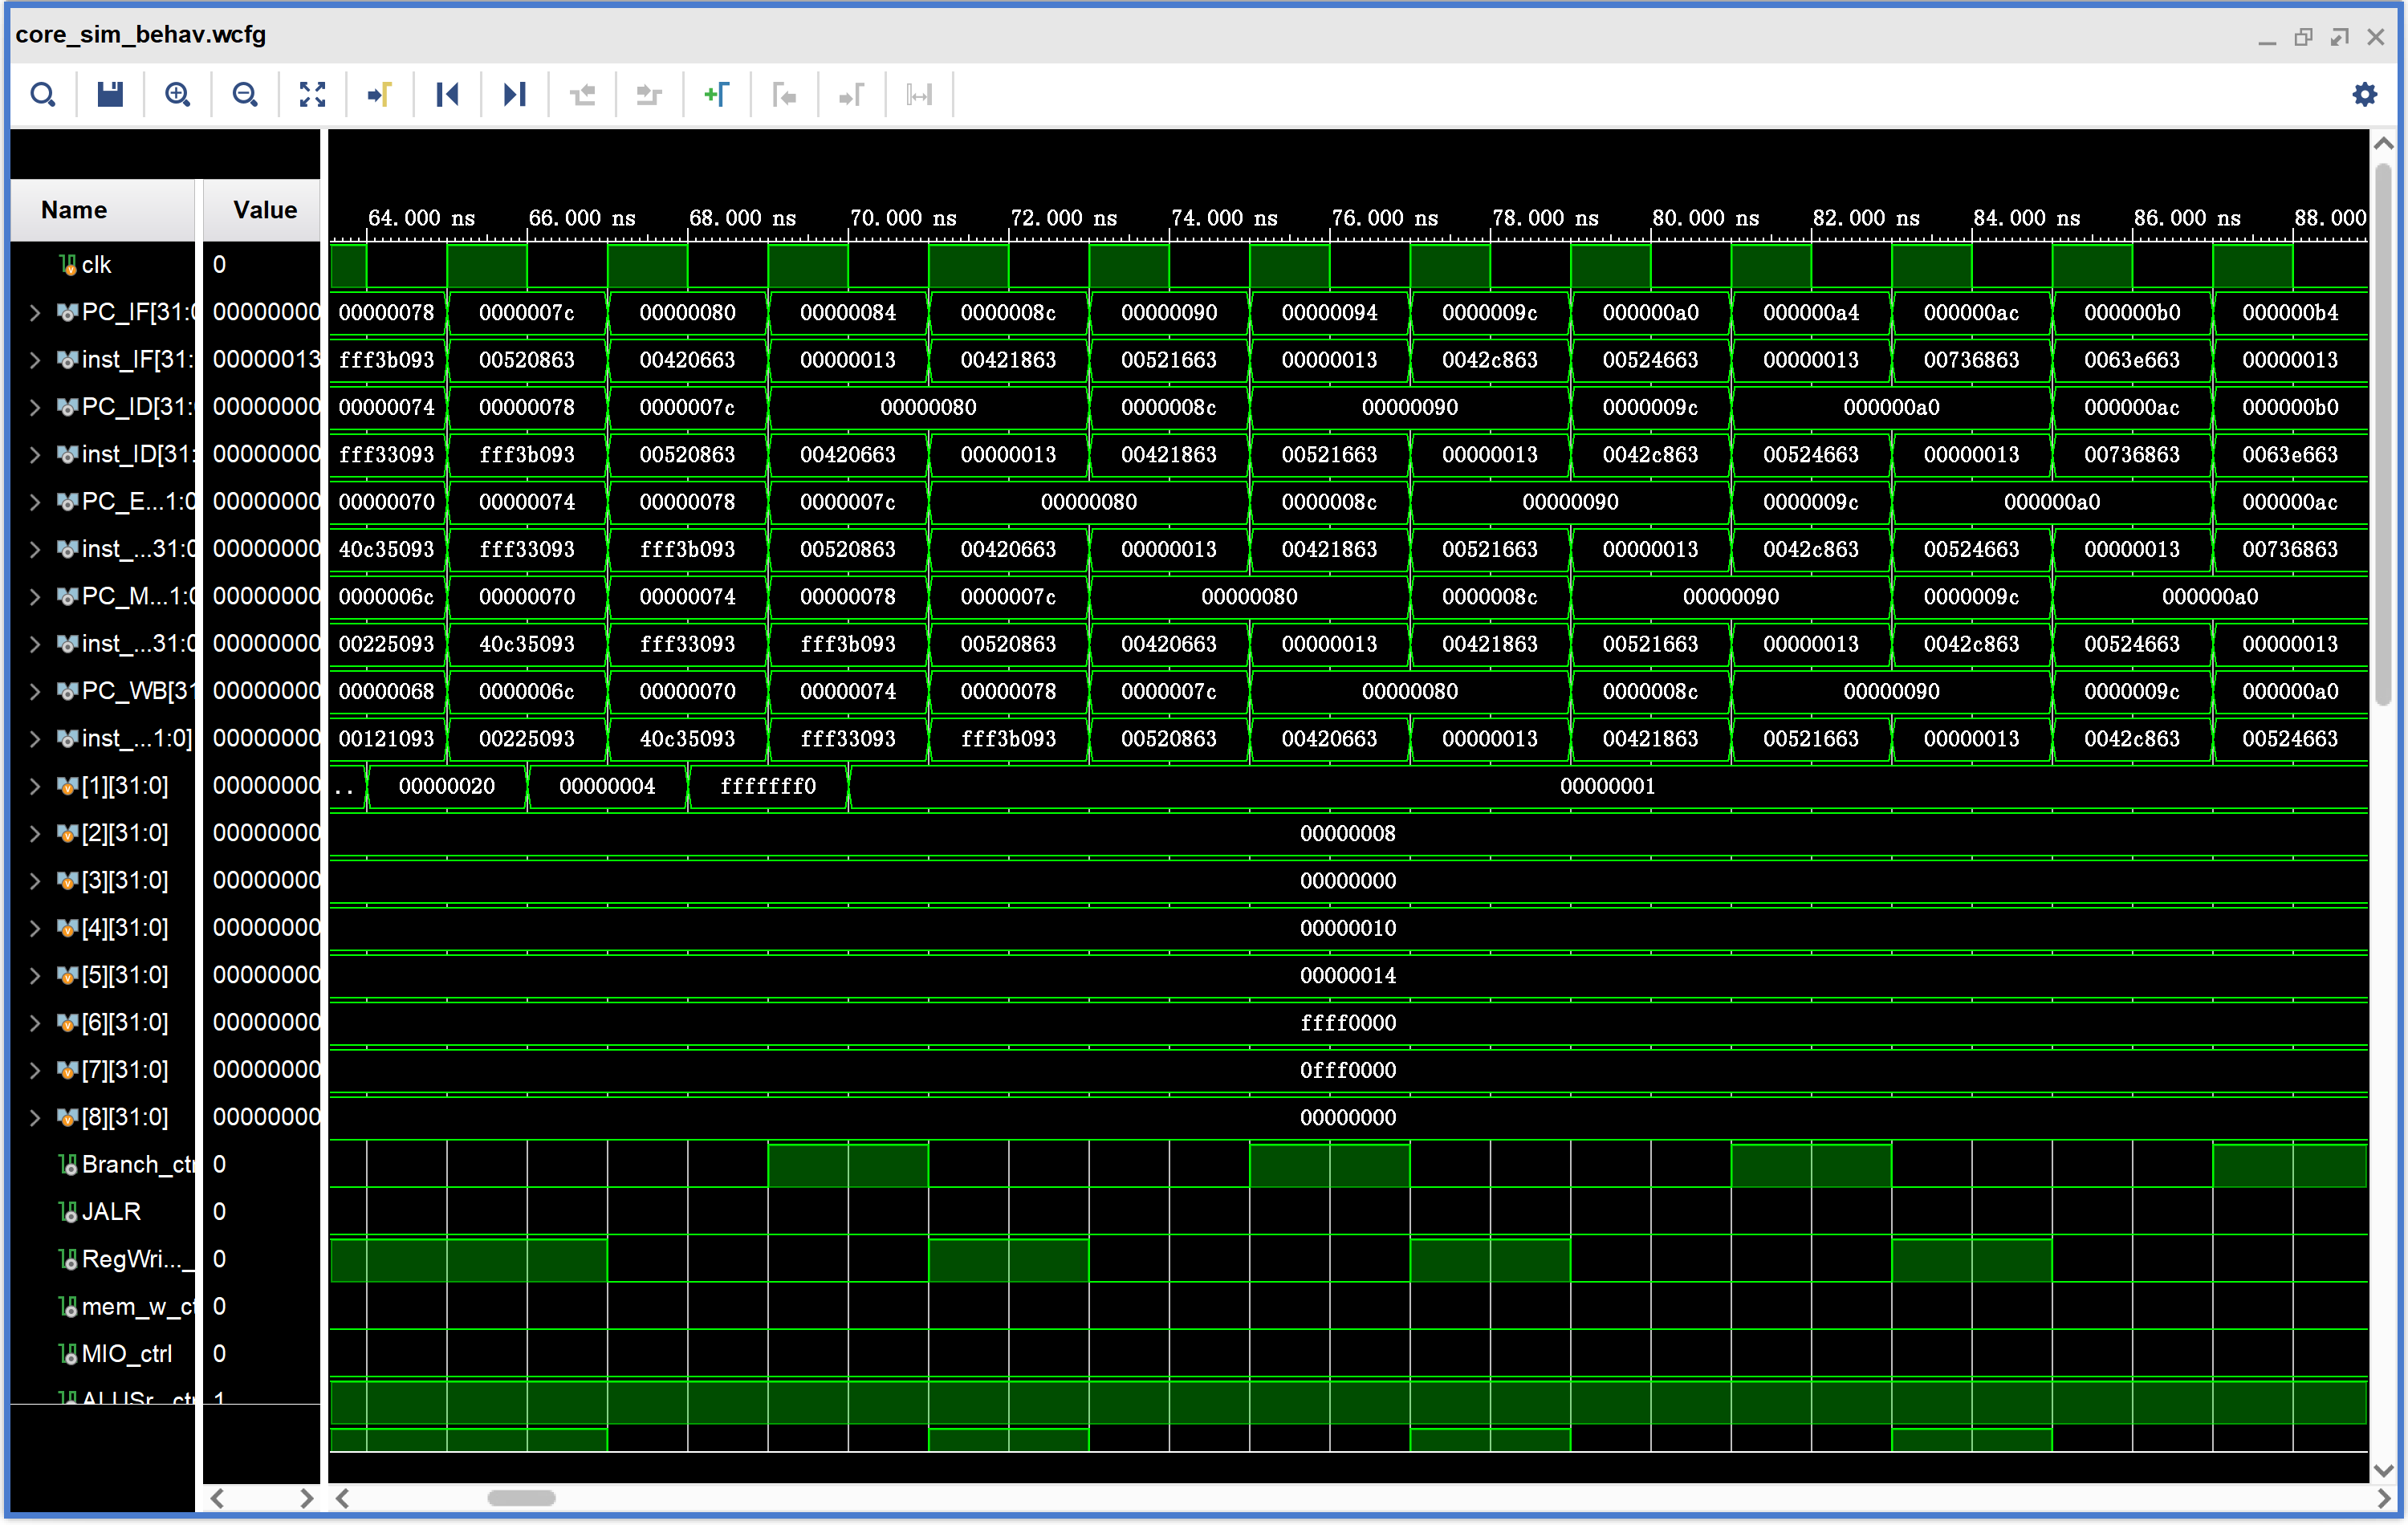
\includegraphics[width=1.0\textwidth]{f2.png} %插入图片,[]中设置图片大小,{}中是图片文件名
	\caption{仿真结果图} %最终文档中希望显示的图片标题
	\label{Fig.4} %用于文内引用的标签
\end{figure}
由图中可以看到branch指令已经实现\\
代码最后,使用jalr指令跳转至代码开头
\begin{figure}
	\centering %图片居中
	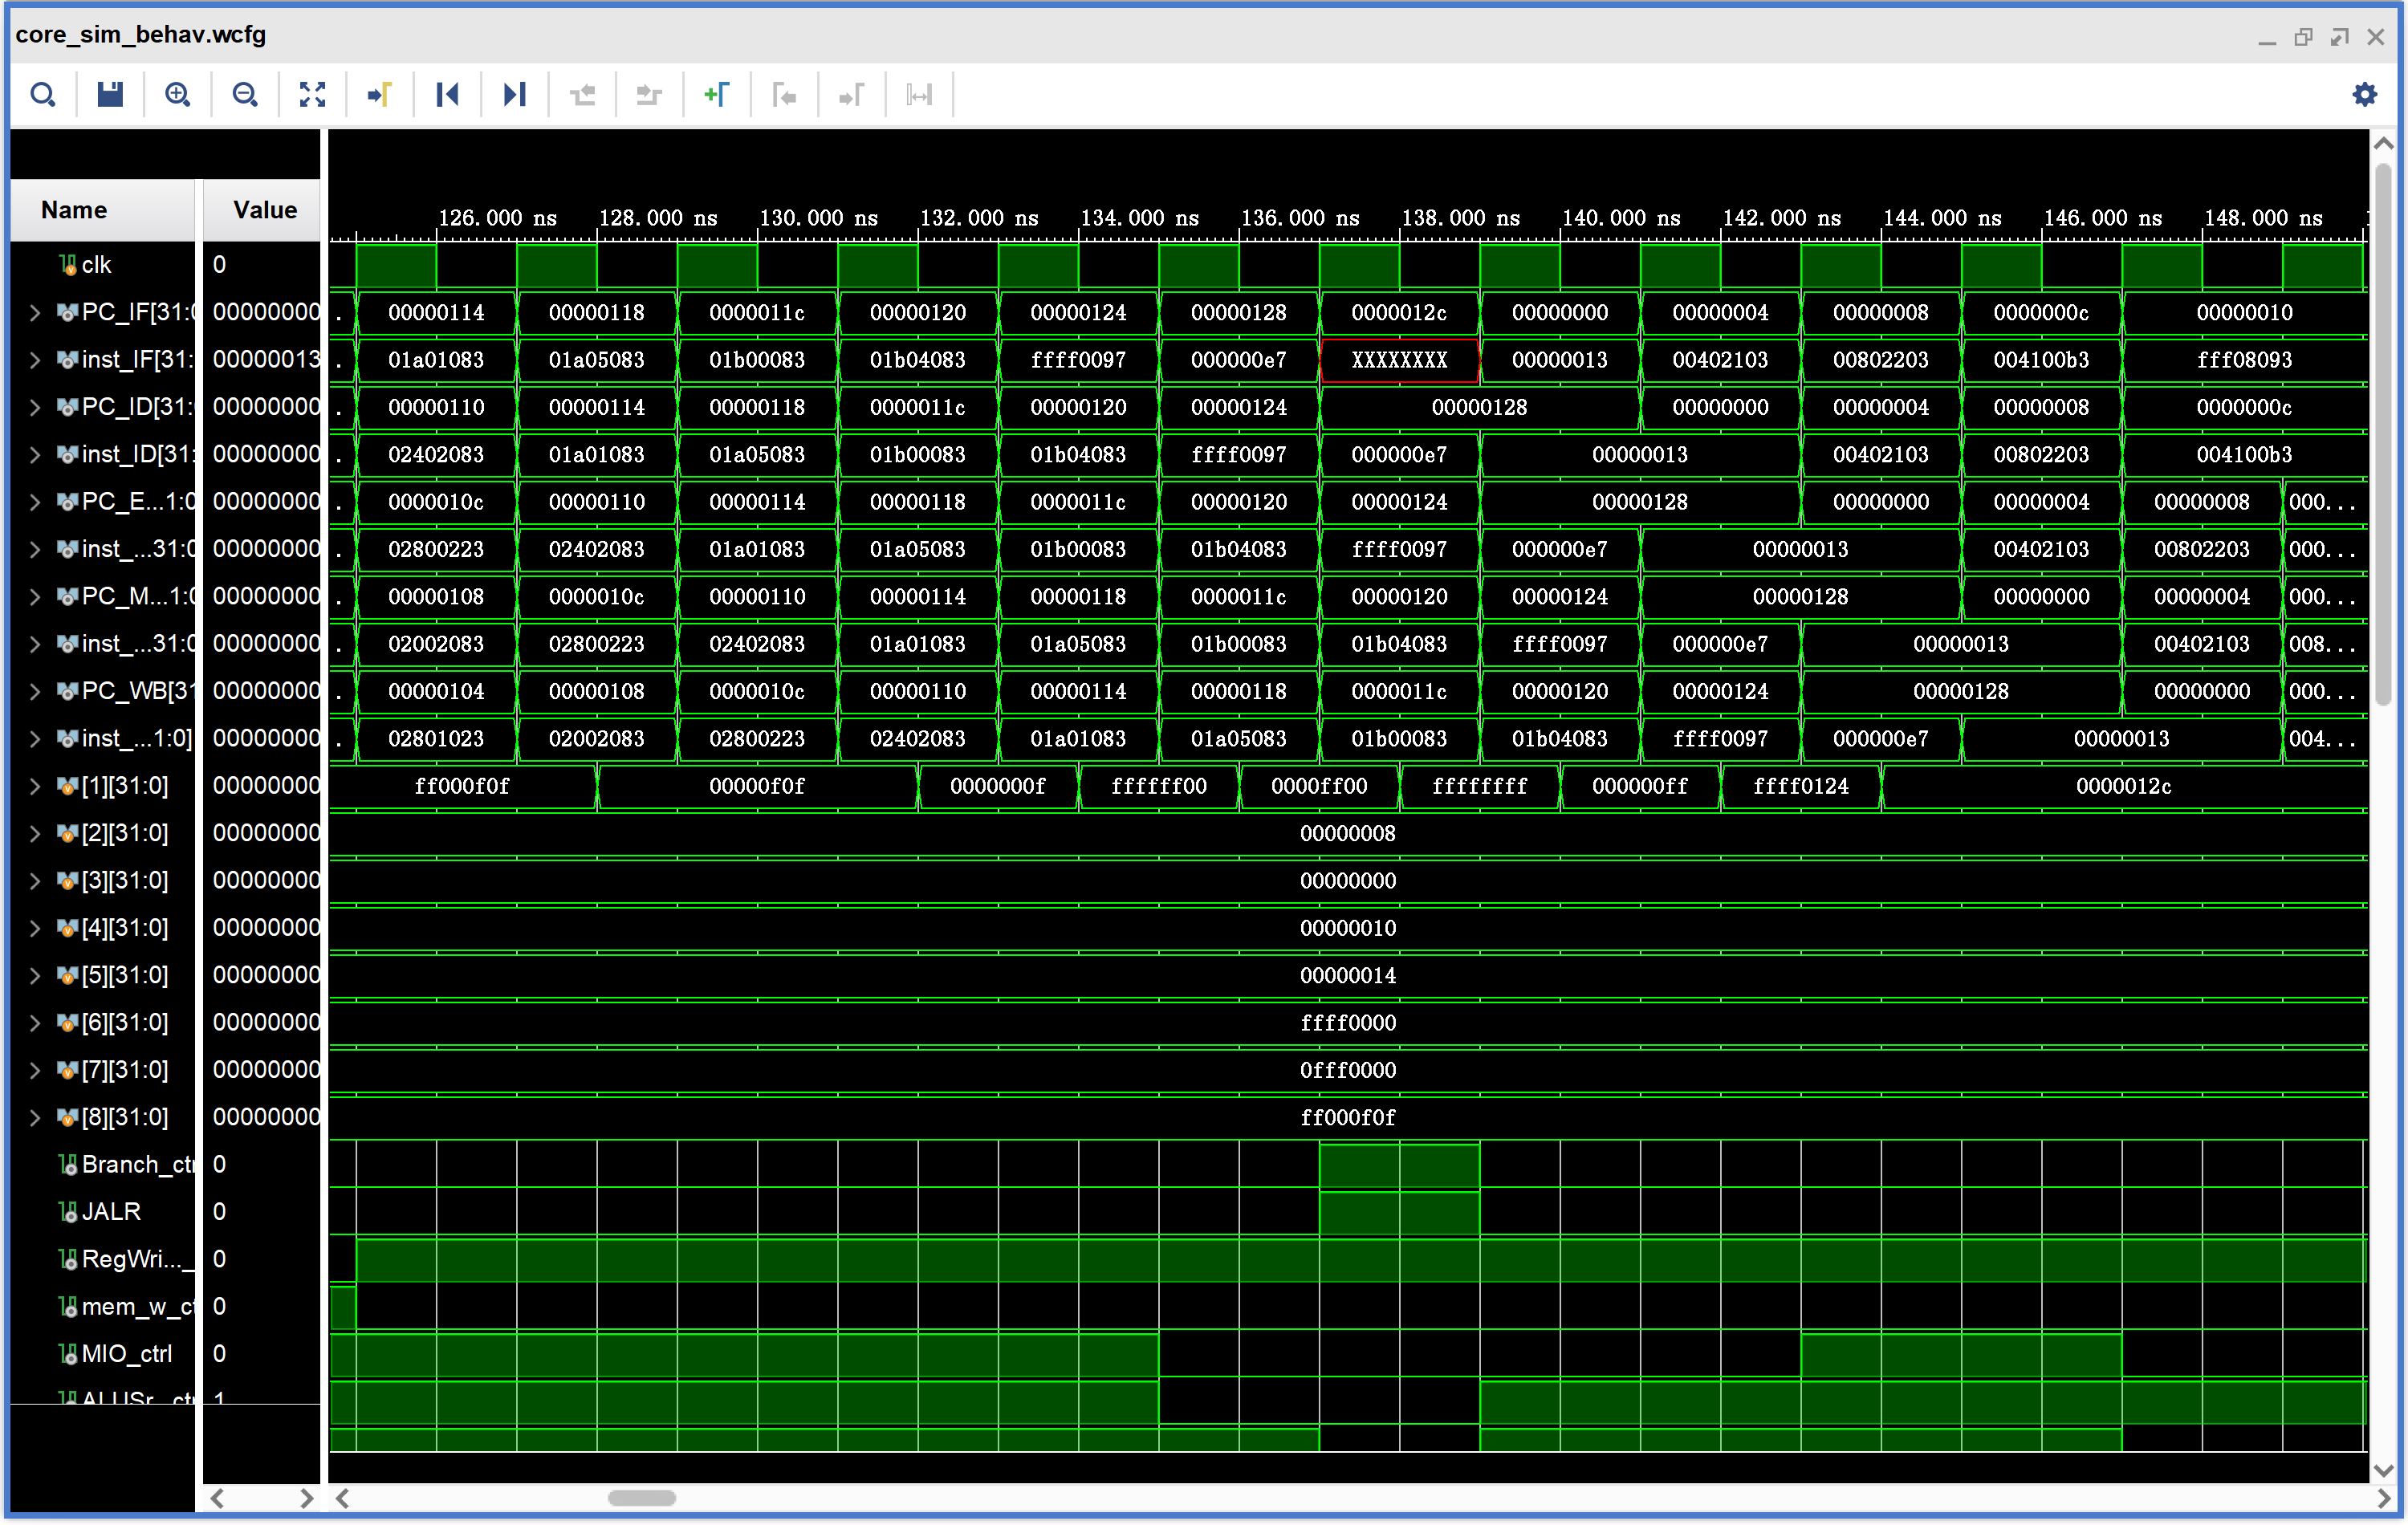
\includegraphics[width=1.0\textwidth]{f3.png} %插入图片,[]中设置图片大小,{}中是图片文件名
	\caption{仿真结果图} %最终文档中希望显示的图片标题
	\label{Fig.5} %用于文内引用的标签
\end{figure}
由图3.5中可以看到,auipc指令与jalr指令的实现没有错误。
\subsection{综合} 选择左侧面板的Run Synthesis或者点击上方的绿色小三角,选择Synthesis
\subsection{实现} 选择左侧面板的Run Implementation或者点击上方的绿色小三角,选择Implementation。值得注意的是执行implementation之前应该确保引脚约束存在且正确,同时之前已经综合过最新的代码。
\subsection{验证设计} 选择左侧面板的Open Elaborated Design,输出的结果如下,根据原理图来判断,基本没有问题
\begin{figure}[H] %H为当前位置,!htb为忽略美学标准,htbp为浮动图形
    \centering %图片居中
    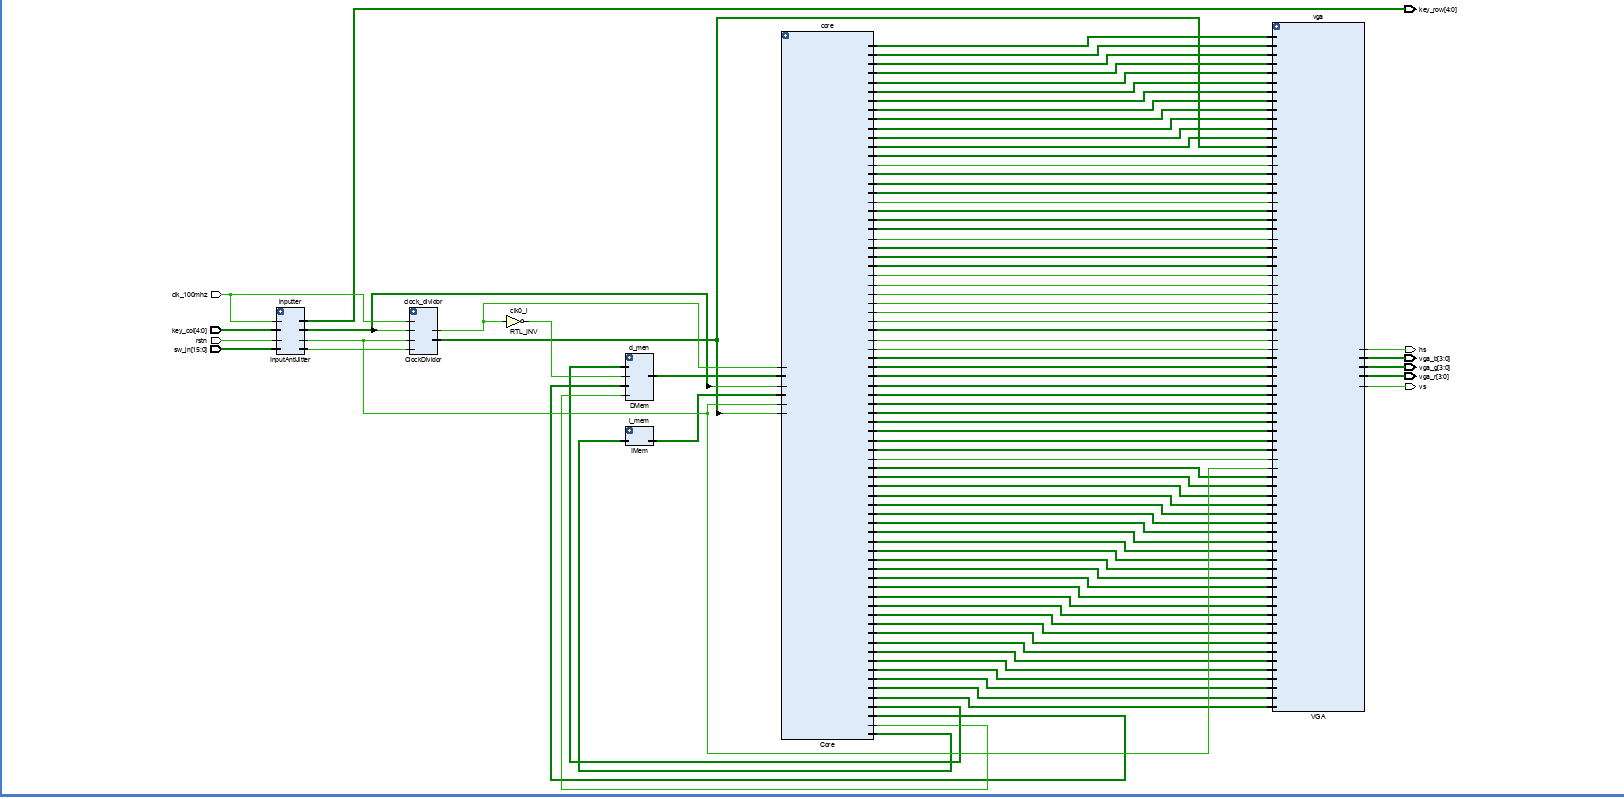
\includegraphics[width=1.0\textwidth]{yanzhen.png} %插入图片,[]中设置图片大小,{}中是图片文件名
    \caption{验证结果图} %最终文档中希望显示的图片标题
    \label{Fig.6} %用于文内引用的标签
\end{figure}
\subsection{生成二进制文件} 选择左侧面板的Generate Bitstream或者点击上上的绿色二进制标志。同时生成Bitstream前要确保:之前已经综合、实现过最新的代码。如没有,直接运行会默认从综合、实现开始。此过程还要注意生成的bit文件默认存放在.runs下相应的implementation文件夹中
\subsection{烧写上板} 点击左侧的Open Hardware Manager $\rightarrow$ 点击Open Target $\rightarrow$ Auto Connect $\rightarrow$ 点击Program Device $\rightarrow$ 选择bistream路径,烧写。验证结果见实验结果部分。
